\documentclass[runningheads,UTF8,article]{comsis2}

\usepackage{graphicx}
\usepackage{color}
\usepackage{appendix}
\newcommand\revised[1]{{\color{black} #1}}

\bibliographystyle{splncs03}
\usepackage{CTEX}

%% Necessary definitions for the running heads
\def\journalissue{Computer Science and Information Systems 00(0):0000--0000}
\def\paperidnum{https://doi.org/10.2298/CSIS123456789X}
\setcounter{page}{1}

\usepackage[pagewise]{lineno}
\linenumbers

\usepackage{hyperref}
\usepackage{verbatim}
\usepackage{graphicx}

\title{A Novel Framework for Automatic Chinese Question Generation Based on Multi-Feature Neural Network Model}

%% Use this if the title is too long for the running heads
\titlerunning{Automatic Chinese Question Generation}

\author{Hai-Tao Zheng\inst{1} \and Jinxin Han\inst{1} \and Jinyuan Chen \inst{1} \and Arun Kumar Sangaiah \inst{2}}

%% Use this the list of authors is too long for the running heads
%\authorrunning{First Author et al.}

\institute{Graduate School at Shenzhen Tsinghua University\\
	China, Shenzhen 518055\\
	\email{zheng.haitao@sz.tsinghua.edu.cn,\\ \{hanjx16,cj-chen13\}@mails.tsinghua.edu.cn}
	\and
	School of Computing Science
	and Engineering VIT University\\
	India, Tamil Nadu Vellore-632014\\
	\email{sarunkumar@vit.ac.in}
}

\begin{document}
	
	\maketitle
	
	\begin{abstract}
		Automatic question generation from text or paragraph is a great challenging task which attracts broad attention in natural language processing. Because of the verbose texts and fragile ranking methods, the quality of top generated questions is poor. In this paper, we present a novel framework Automatic Chinese Question Generation (ACQG) to generate questions from text or paragraph. In ACQG, we use an adopted TextRank to extract key sentences and a template-based method to construct questions from key sentences. Then a multi-feature neural network model is built for ranking to obtain the top questions. The automatic evaluation result reveals that the proposed framework outperforms the state-of-the-art systems in terms of perplexity. In human evaluation, questions generated by ACQG rate a higher score.
		
		
		\vspace{6pt}\textbf{Keywords:}  Chinese Question Generation, TextRank, Multi-Feature Neural Network Model .
	\end{abstract}
	
	\section{Introduction}
	
	
	
	
	Question generation aims to create natural questions from a given text or paragraph, and there are a lot of demands in the field of natural language processing, such as \revised{reading comprehension} \cite{heilman2010good,DBLP:journals/corr/DuSC17,duke2008effective}, developing as a chatbot component to request feedback \cite{colby1971artificial}, and improving mental health \cite{mostafazadeh2016generating}. Besides, question generation systems can aid in the development of annotated datasets for question answering \cite{rajpurkar2016squad}. The existing question generation approaches can be categorized as template-based \cite{mostow2009generating,lindberg2013generating,heilman2010good}, semantic-based \cite{Kunichika2001AutomatedQG,infusing,mazidi2014linguistic}, and  sequence-to-sequence-based \cite{mostafazadeh2016generating,serban2016generating,DBLP:journals/corr/DuSC17}. The success of these approaches hinges critically on the existence of well-designed rules for declarative-to-interrogative sentence transformation or a powerful labeled dataset.
	
	However, the main points or events of text only contain in few key sentences. Authors express their emotions or points indirectly, so the texts always exhibit complex structure and long content. The verbose texts make existing approaches generate many unimportant questions, which are unacceptable for users. 
	In addition, the fragile ranking methods do not take enough features into account, such as the $n$-gram score in question, answer's location position in original sentence and so on. As a result, the key questions do not always appear in the front rank of outputs. 
	
	
	%To improve the performance of the state-of-the-art Heilman and Smith \cite{heilman2010good} system,
	
	To address these issues, we introduce an Automatic Chinese Question Generation (ACGQ) approach. Since the verbose text content is not a good input for question construction, we firstly extract key sentences from text, and locate the main points. Next, a template-based question construction model is built to generate questions from declarative-to-interrogative sentence. Finally, a multi-feature neural ranking model is proposed to rank the generated questions.
	
	The main contributions of our work are listed as follows:
	\begin{enumerate}
		\item {We develop an adapted TextRank model to identify the key sentences of text and filter verbose sentences from source.}
		\item{We design a multi-feature neural network model to rank all generated questions and obtain more acceptable questions in the front rank.}
		\item{We conduct extensive experiments and the results show that our framework achieves a better performance \revised{compared to} the state-of-the-art systems in terms of perplexity and human evaluation measurement.}
	\end{enumerate}
	
	
	The remainder of the paper is organized as follows. In section 2, we review related work on question generation. Section 3 introduces an overview of our model and a detailed description of each component. Section 4 details the experiments setup and their results. Section 5 concludes this paper and puts forward future work. 	
	
	
	
	\section{Related Work}
	
	% 介绍点其他类型方法的工作,已经总结过得 语法方面的工作
	
	The concept of question generation was presented dating back to 1976 by Wolfe \cite{wolfe},	which has attracted attention of the natural language generation community in recent years since the work of Rus et al. \cite{rus2010first}.
	
	
	Most works tackle this task with a template-based approach. Generally, they transform the input sentence into its syntactic representation, which then are used to generate an interrogative sentence. A lot of researches have focused on manually constructing question templates, and then applying them to generation questions \cite{mostow2009generating,lindberg2013generating,heilman2010good}. 
	Mostow et. al \cite{mostow2009generating} proposed a self-questioning strategy for \revised{reading comprehension}, in this strategy, three templates are firstly built to generate questions about \emph{what,how,why}. Lindberg et al.\cite{lindberg2013generating} adopted a templated-based method, using predominately semantic information.
	This method bases on semantic patterns, which cast a wide syntactic net and a narrow semantic net. Then they construct questions according to the parser and templates. Heilman and Smith \cite{heilman2010good} introduced an overgenerate-and-rank approach. \revised{Their framework can be viewed as a two-step process for question generation.  In the first step, it transforms the input sentence into a simpler sentence, which is transformed into a more succinct question. In the second step, the declarative sentence is transformed into sets of questions by a sequence of well-defined syntactic and lexical transformations. It identifies the answer phrases which may be targets for WH-movement and converts them into question phrases}. Yao et al. \cite{yao} and Becker et al.\cite{becker} both followed this strategy. However, this kind of approaches does not work well when the input text is verbose, and the result is rough and redundant.
	
	
	
	Another view is generating question based on semantic, the semantic role labels include subject, predicate verb, object, tense and so on. The semantic roles are used to determine the interrogative pronoun for the generated question \cite{Kunichika2001AutomatedQG,infusing,mazidi2014linguistic}. Kunichika et al. \cite{Kunichika2001AutomatedQG} carried out their work in automatically generating reading comprehension questions, the questions included both syntax and semantic questions.
	Mazidi and Nielsen \cite{mazidi2014linguistic} uses semantic pattern recognition to crate questions of varying depth and type for self-study. Generation patterns specify the text, verb forms and semantic arguments form the source sentence to form the question. Mazidi and Tarau \cite{infusing} focused on the frequency of pattern sentence occurrences and the consistency of semantic information conveyed by the pattern to generate questions, this method could generate questions in a low dimension. Such approaches generate a wider variety of questions which are not as closely bound to original text, and there are syntax errors in some questions.
	
	
	Nowadays neural network with word embedding can be effectively applied to the natural language processing task with highly accurate results \cite{NIPS2016_6469,DBLP:journals/corr/VinyalsTBE14}. Mostafazadeh et al. \cite{mostafazadeh2016generating} introduced visual question generation to explore the deep connection between language and vision. Serban et al. \cite{serban2016generating} proposed generating simple factoid questions from logic triple (subject, relation, object). Their task tackles mapping from structured representation to natural language text, and their generated questions are consistent in terms of format. Xinya Du et.al \cite{DBLP:journals/corr/DuSC17} built a bigger dataset for text\&question based on SQuAD \footnote{https://rajpurkar.github.io/SQuAD-explorer/}, and trained a sequence to sequence network to generate questions on level on word and paragraph. These supervised methods need a large scale of labeled data and cost much time to train the network, which are not a good way to handle question generation problem for a rare of Chinese dataset.
	
	
	\revised{To conclude, most of the existing question generation models are based on full texts, leading to generate some redundant questions. in addition, the fragile ranking methods do not take enough features into account and many useless questions are generated. In order to improve the performance of Chinese question generation, ACQG identifies the key sentences in texts and utilizes multiple features for question ranking.}
	
	
	
	\section{The Framework of Automatic Chinese Question Generation}
	The goal of ACQG is to generate more acceptable questions from text or paragraph. The framework is shown in Fig.~\ref{framework}. This involves 1) identifying the key sentences of text with an adapted TextRank. 2) constructing questions according to rule-based templates. 3) ranking questions with a multi-feature neural network model.
	\begin{figure}[h]
		\centering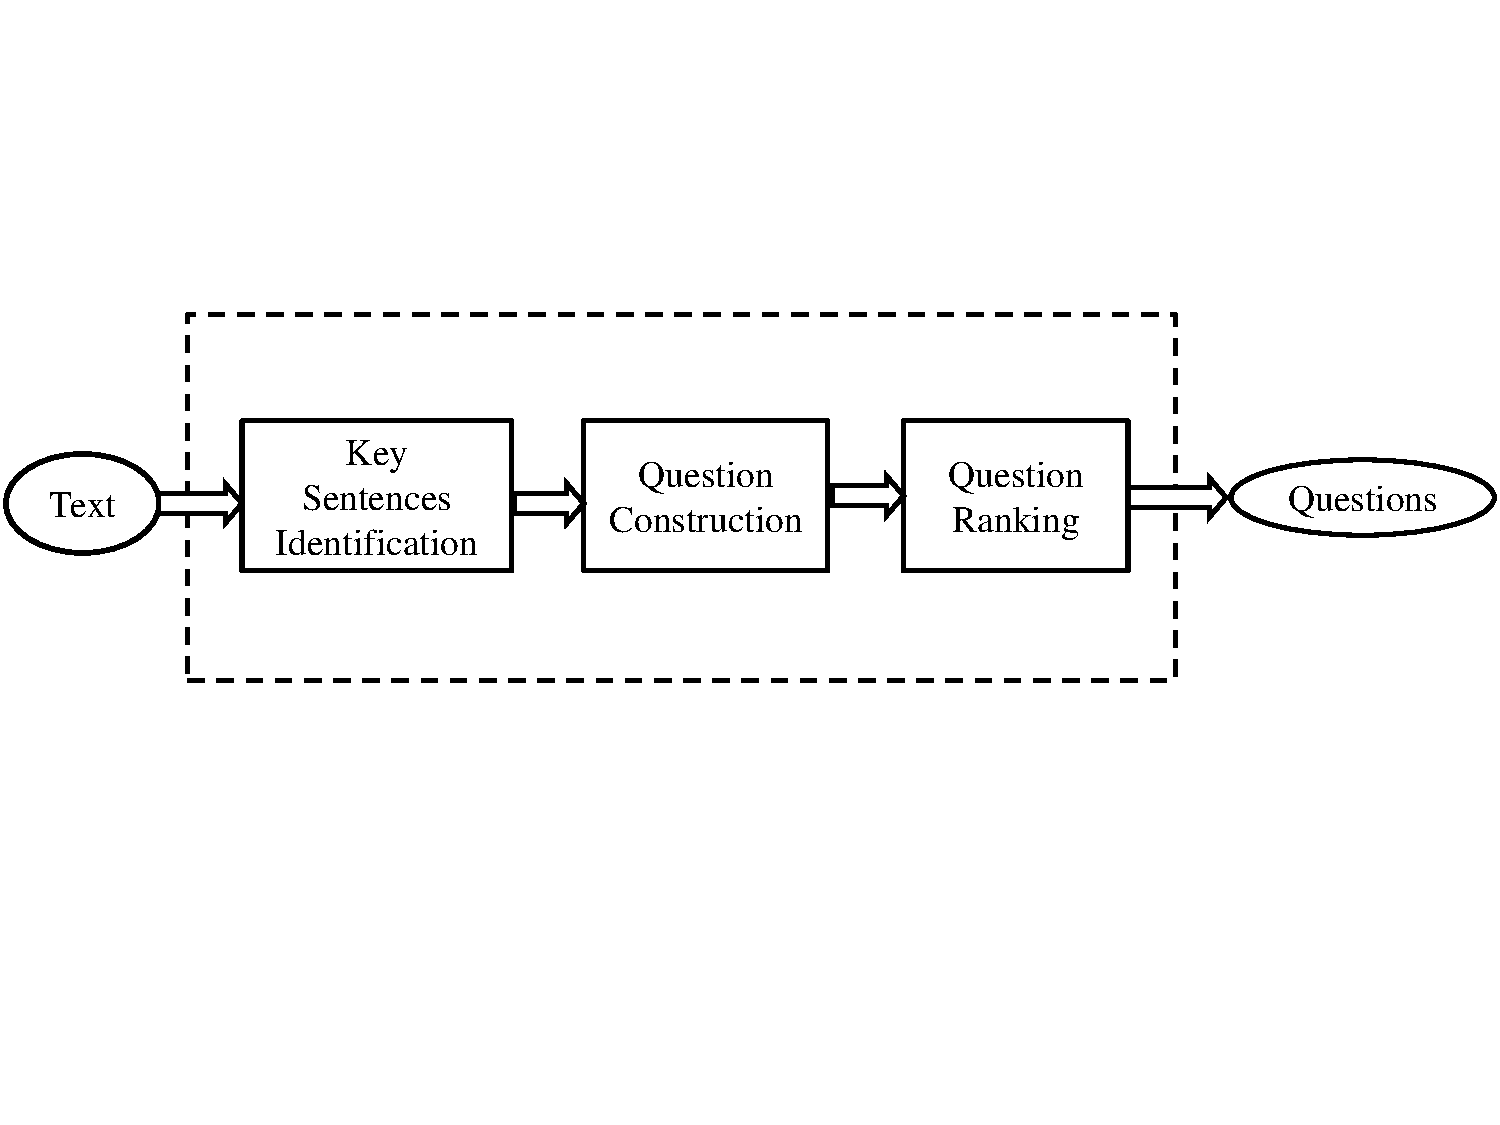
\includegraphics[width=0.7\columnwidth]{framework.pdf}
		\caption{Overview of Automatic Chinese Question Generation Framework}
		\label{framework}
	\end{figure} 
	
	
	
	
	
	\subsection{Key Sentences Identification}
	
	To identify the key sentences from text or paragraph, we use an adapted TextRank method. Graph-based ranking algorithm is a common measure to extract the key content in web \cite{zhu2016deep,mihalcea2004graph}. A similar method called TextRank \cite{textrank} can be applied to extract summary from document. In this work, we use an adapted TextRank to identify key sentences from text, which converts text to a graph and calculates the score of each sentence node. When the score of a sentence is greater than the set threshold $ \theta $, the sentence will be selected. 
	The original TextRank employs the BM25\footnote{https://en.wikipedia.org/wiki/Okapi\_BM25} to compute the similarity of sequence, whereas it has many manual setting parameters leading to inefficient results. 
	Therefore, we use the cosine similarity replaced in our method. The details are described as follows.
	
	The input text $ T $ is divided into some sentences with different terminators (e.g. `。',`!',`?'). $ T=\{S_0,S_1,...S_i,...,S_n\}$, $ S_i  $ represents a sentence in $ T $, $ n $ is the total number of sentences in $ T $. Then we segment $ S_i $ into words. $ S_i=\{w_0,w_1,...,w_k...,w_m\}$, $ w_k $ represents a word in $ S_i  $, $ m  $ is the total number of words in $ S_i  $ . 
	
	We introduce Term Frequency–Inverse Document Frequency \cite{tfidf} to quantify each word, where $ TF(w_k) $ is the frequency of $ w_k $ in $ T $, $ IDF(w_k) =log \frac{||T||}{||w_k \in T||}$ is an inverse word frequency in total texts, $||T||$ is the total number of texts in dataset. So a sentence can be represented to a word vector. The similar score is computed by Equation.~\ref{simality}.
	\begin{equation}
		sim_{ij} = sim(S_i,S_j)=\frac{\sum_{w_v \in S_i \cap{S_j}}(TF(w_v)IDF(w_v))^2}{|S_i||S_j|}
		\label{simality}
	\end{equation}
	
	For a given sentence $ S_i $, $In(S_i) $ is the previous sentences, $ Out(S_i) $ is the subsequent sentences. The score of $ S_i $ is computed using the Equation.~\ref{score}.
	\begin{equation}
		WS(S_i)=(1-d)+d*\sum_{S_j \in In(S_i)} \frac{sim_{ji}}{ \sum_{S_k \in Out(S_j) sim_{jk}}}WS(S_j)
		\label{score}
	\end{equation}
	\noindent Where $ d $ is a parameter that is set between 0 and 1. 
	
	When the algorithm finished, a score associates with each sentence, and it expresses the importance of sentence in text. Whether the sentence is selected or not depends on this score.
	
	\subsection{Question Construction}
	In this section, we describe how to construct questions from sentence. In particular, we focus on the structure and relation between words to construct questions. We design different rule-based templates to construct targeted questions from the parser tree.
	
	Firstly, we design 5 general templates. If an input sentence contains location, person, noun, or time finding them by Named Entity Recognition (NER) , we construct \emph{Where}, \emph{Who}, \emph{What} or \emph{When} type of question. If there is adjective around noun, we construct \emph{How} question. Then we replace a question type with the named entity to generate a question by declarative-to-interrogative. A good performance of NER is important for the type of question. To ensure the quality of tokenize and NER, we expand the annotators by getting neologisms from Wikipedia\footnote{https://en.wikipedia.org/wiki/Main\_Page} regularly.
	
	Secondly, we design more templates aiming at generating targeted questions. Parser tree describes the relationship among verb, subject, object, and so on. We utilize it to analyze each sentence, and edit some templates learning from text to generate targeted questions. The templates are listed as follows.
	\begin{enumerate}
		\item{\emph{number} question\,:\, (QP $ < $ CD =number  $ < $ CLP)}
		\item{\emph{rank} question\,:\, (QP $ < $ OD=number)}
		\item{\emph{if-cause} question \,:\, ((IP$ | $ PP=reason $ << $ 由于(because of) $ | $ 因为(because)) ..(IP$ | $ PP$ | $ VP)$ |<< $ (IP$ | $ PP $ | $VP $ << $ 所以(so) $ | $ 于是(so that)))}
		\item{\emph{relative-cause} question\,:\, ((( IP $ | $ PP=front $ << $ 虽然(though)) .IP=however )$ | $ $<<$ (IP $|$ PP=front(IP $|$ PP $|$ VP=however $<<$ 但是(but) $|$ 但(but)))) }
		
		\item{\emph{color} question\,:\, (QP $ < $ NP=JJ $ < $ NP) }
		
	\end{enumerate}
	
	IP, PP, and VP represent different tag of words. A dot means subsequent follow and a left shaped arrow means an immediate subtree relation. These templates guide to search possible answer phrases on the parser tree. Once a subtree matches any template, a question will be constructed.
	\revised{
	In order to have a better understanding of each template, we list some examples in Table.~\ref{example}.}
	
	
	\begin{table}[!ht]
		\centering
		\caption{The Template Examples}
		\setlength\tabcolsep{0.5em}
		\label{example}
		\begin{tabular}{|p{25pt}|p{155pt} | p{150pt} |}
			\hline
			Type& Sentence & Question \\
			\hline
			\emph{Who} & 刘佩英任安吉斯中国首席商务官。(Peiying Liu acts as the China chief commercial officer of Angis.) & 谁任安吉斯中国首席商务官?(Who acts as the China chief commercial officer of Angis?)\\
			\hline
			\emph{When} & 2017年退休人员基本养老金上调。(The basic pension of retirees will increase in 2017.) & 何时退休人员基本养老金上调?(When will the basic pension of retires increase?)  \\
			\hline
			\emph{Where} & 二战时日本曾在越南制造大饥荒。(Japan had created a famine in Vietnam during World War II.)& 二战时日本曾在哪里制造大饥荒?	(Where had Japan created a famine during World War II?) \\
			\hline
			\emph{rank}& 昆仑鸿星取关键一胜跃居东区第六位 (Kunlun Hongxing becomes the Sixth in the East by taking a key victory.)& 昆仑鸿星取关键一胜跃居东区第几位?(What is the ranking of Kunlun Hongxing in the East by taking a key victory?)\\
			\hline
			\emph{number}& 亚泰2000万镑交易震惊世界!(The transaction of Yatay 20 million pound shocked the world.)& 亚泰多少镑交易震惊世界?(What`s the amount of the transaction of Yatay shocked the world?) \\
			\hline
			\emph{if-cause}& 因为人工智能快速发展,人们的生活方式得到巨大改变。(Because of the rapid development of artificial intelligence, people`s lifestyle has been greatly changed.)&	人们的生活方式得到巨大改变,因为什么?(What makes people's lifestyle have been change greatly? )\\
			\hline
			\emph{relative-cause}& 春运将至,铁道部门虽然提前发售车票,但买票难的问题仍然存在。	(As Spring Festival is coming, the railway department has sold tickets in advance, but it is still difficult to buy a ticket. )&春运将至,铁道部门虽然提前发售车票,但怎么样?(As Spring Festival is coming, what`s happened when the railway department has sold tickets in advance?)\\
			
			\hline
			\emph{color} & 天气红色预警发布后,学校需要停课。 (After the weather red warning released, classes will be suspended.) &   什么颜色天气预警发布后,学校需要停课? (Classes will be suspended after which color warning released?) \\ 
			\hline
		\end{tabular}
	\end{table}	
	
	
	
	\iffalse
	\begin{table}[!ht]
		\centering
		\caption{The Template Examples}
		\setlength\tabcolsep{0.5em}
		\label{example}
		\begin{tabular}{|p{25pt}|p{125pt} | p{120pt} |p{45pt}|}
			\hline
			Type& Sentence & Question & Answer \\
			\hline
			\emph{Who} & 刘佩英任安吉斯中国首席商务官。(Peiying Liu acts as the China chief commercial officer of Angis.) & 谁任安吉斯中国首席商务官?(Who acts as the China chief commercial officer of Angis?)& 刘佩英    (Peiying Liu)\\
			\hline
			\emph{When} & 2017年退休人员基本养老金上调。(The basic pension of retirees will increase in 2017.) & 何时退休人员基本养老金上调?(When will the basic pension of retires increase?) & 2017年 (In 2017) \\
			\hline
			\emph{Where} & 二战时日本曾在越南制造大饥荒。(Japan had created a famine in Vietnam during World War II.)& 二战时日本曾在哪里制造大饥荒?	(Where had Japan created a famine during World War II?) & 越南(In Vietnam)\\
			\hline
			\emph{rank}& 昆仑鸿星取关键一胜跃居东区第六位 (Kunlun Hongxing becomes the Sixth in the East by taking a key victory.)& 昆仑鸿星取关键一胜跃居东区第几位?(What is the ranking of Kunlun Hongxing in the East by taking a key victory?)& 第六(the Sixth)\\
			\hline
			\emph{number}& 亚泰2000万镑交易震惊世界!(The transaction of Yatay 20 million pound shocked the world.)& 亚泰多少镑交易震惊世界?(What`s the amount of the transaction of Yatay shocked the world?)& 2000万(20 million) \\
			\hline
			\emph{if-cause}& 因为人工智能快速发展,人们的生活方式得到巨大改变。(Because of the rapid development of artificial intelligence, people`s lifestyle have been greatly changed.)&	人们的生活方式得到巨大改变,因为什么?(What makes people's lifestyle have been change greatly? )&	人工智能快速发展(The rapid development of artificial intelligence)\\
			\hline
			\emph{relative-cause}& 春运将至,铁道部门虽然提前发售车票,但买票难的问题仍然存在。	(As Spring Festival is comming, the railway department has sold tickets in advance, but it is still difficult to buy a ticket. )&春运将至,铁道部门虽然提前发售车票,但怎么样?(As Spring Festival is comming, what`s happened when the railway department has sold tickets in advance?)&	买票难的问题仍然存在(It is still difficult to buy a ticket )\\
			
			\hline
			\emph{color} & 天气红色预警发布后,学校需要停课。 (After the weather red warning is released, the schools need to be closed.) &   什么颜色天气预警发布后,学校需要停课? (After what color whether warning is released, the schools need to be closed?)  & 红色 (red color)\\ 
			\hline
		\end{tabular}
	\end{table}
	

		For example, given the input text, ``2014年因埃博拉病毒大肆蔓延,造成多地人员伤亡,但被切断传播链后疫情得到控制。(There are many casualties because of the violent spread of Ebola in 2014. But the epidemic is under control after interrupting the chains of transmission.)", many questions are generated as shown in Table.~\ref{questions}. \revised{Besides, we present an example of each template for better understanding in Appendix.}
		
		
	
	\begin{table}[!th]
		
		\centering
		\caption{The Generated Questions Table }
		\label{questions}
		\setlength\tabcolsep{0.5em}
		
		\begin{tabular}{|p{55pt}|p{250pt}|}
			\hline
			Type  & Example\\
			\hline
			\emph{When} & 埃博拉病毒大肆蔓延在什么时候?\\
			&(When did the violent spread of Ebola?)\\         
			\emph{What} & 因什么大肆蔓延,造成到底人员伤亡?\\
			& (What spreads violently causing many casualties?)\\       
			\emph{if-cause} &  为什么多地出现人员伤亡?\\
			& (Why are there many casualties?)\\
			\emph{relative-cause} & 因埃博拉病毒大肆蔓延,造成多地人员伤亡,但怎么样了?\\
			&(There are many casualties, because of the violent\\
			& spread of Ebola. But what happened after that?)\\
			\hline
			
		\end{tabular}	
		
	\end{table}
	\fi
	
	
	
	
	
	
	\subsection{Question Ranking}
	%We propose a simple and effective method to remedy the duplicate issue. If any of output questions own the similar answer or content with another one, we remove one of them to ensure that the question includes no duplicate. 
	
	After the two processes above, we can obtain lots of questions, while these questions are sorted arbitrarily and the key questions do not always appear in the front rank of outputs. We build a multi-feature neural ranking model to select the top key questions. We import twelve features from the generated questions and text, shown in Table.~\ref{features}, and design a multi-feature neural network model to rank them. This is an appropriate solution to the multiple features problem without manual intervention. 
	\begin{table}[!th]
		\centering
		\caption{All Features to Rank}
		\label{features}
		\setlength\tabcolsep{0.5em}
		\begin{tabular}{|p{200pt}|}
			\hline
			\textbf{Feature} \\
			\hline
			$ f1 $\,:\,number of tokens in question and answer\\ 
			$ f2 $\,:\,number of named entity in question \\   
			$ f3 $\,:\,type of question \\ 
			$ f4 $\,:\,score of key sentence  \\ 
			$ f5 $\,:\,answer's location position in original sentence  \\ 
			$ f6 $\,:\,the unigram, bigram and trigram score of question\\     			
			$ f7 $\,:\,percentage of keywords in question \\
			$ f8 $\,:\,stopwords density in question\\	
			$ f9 $\,:\,noun density in question\\
			$ f10 $\,:\,verb density in question \\
			
			$f11$\,:\,information gain \\
			$f12$\,:\,TF-IDF score   \\
			\hline 
		\end{tabular}	
	\end{table}
	
	
	
	
	
	%{介绍一下各种指标为啥要被选择
	%The ranking algorithm could certainly be improved with more useful features, as Table \ref{features}, but we do not claim that all features are initial to be selected. 
	As shown in Table.~\ref{features}, we select twelve features about generated questions and original text.
	Additionally, the features $f1
	\scriptsize{\sim}f5$ are basic information of question and answer. $f6$ are the $n$-gram scores in question sequence, which provide rich contextual information. $f7$ is used to compute the keywords percentage in question. $ f8 \scriptsize{\sim}f10$ are different tags of word distribution in question, which indicate the structure of question sequence. $ f11$ is a probability data, which represents the uncertainty of sentence. $ f12$ is a numerical statistic measure that is a popular sentence-weighting scheme. 
	
	\begin{figure}[!ht]
		\centering
		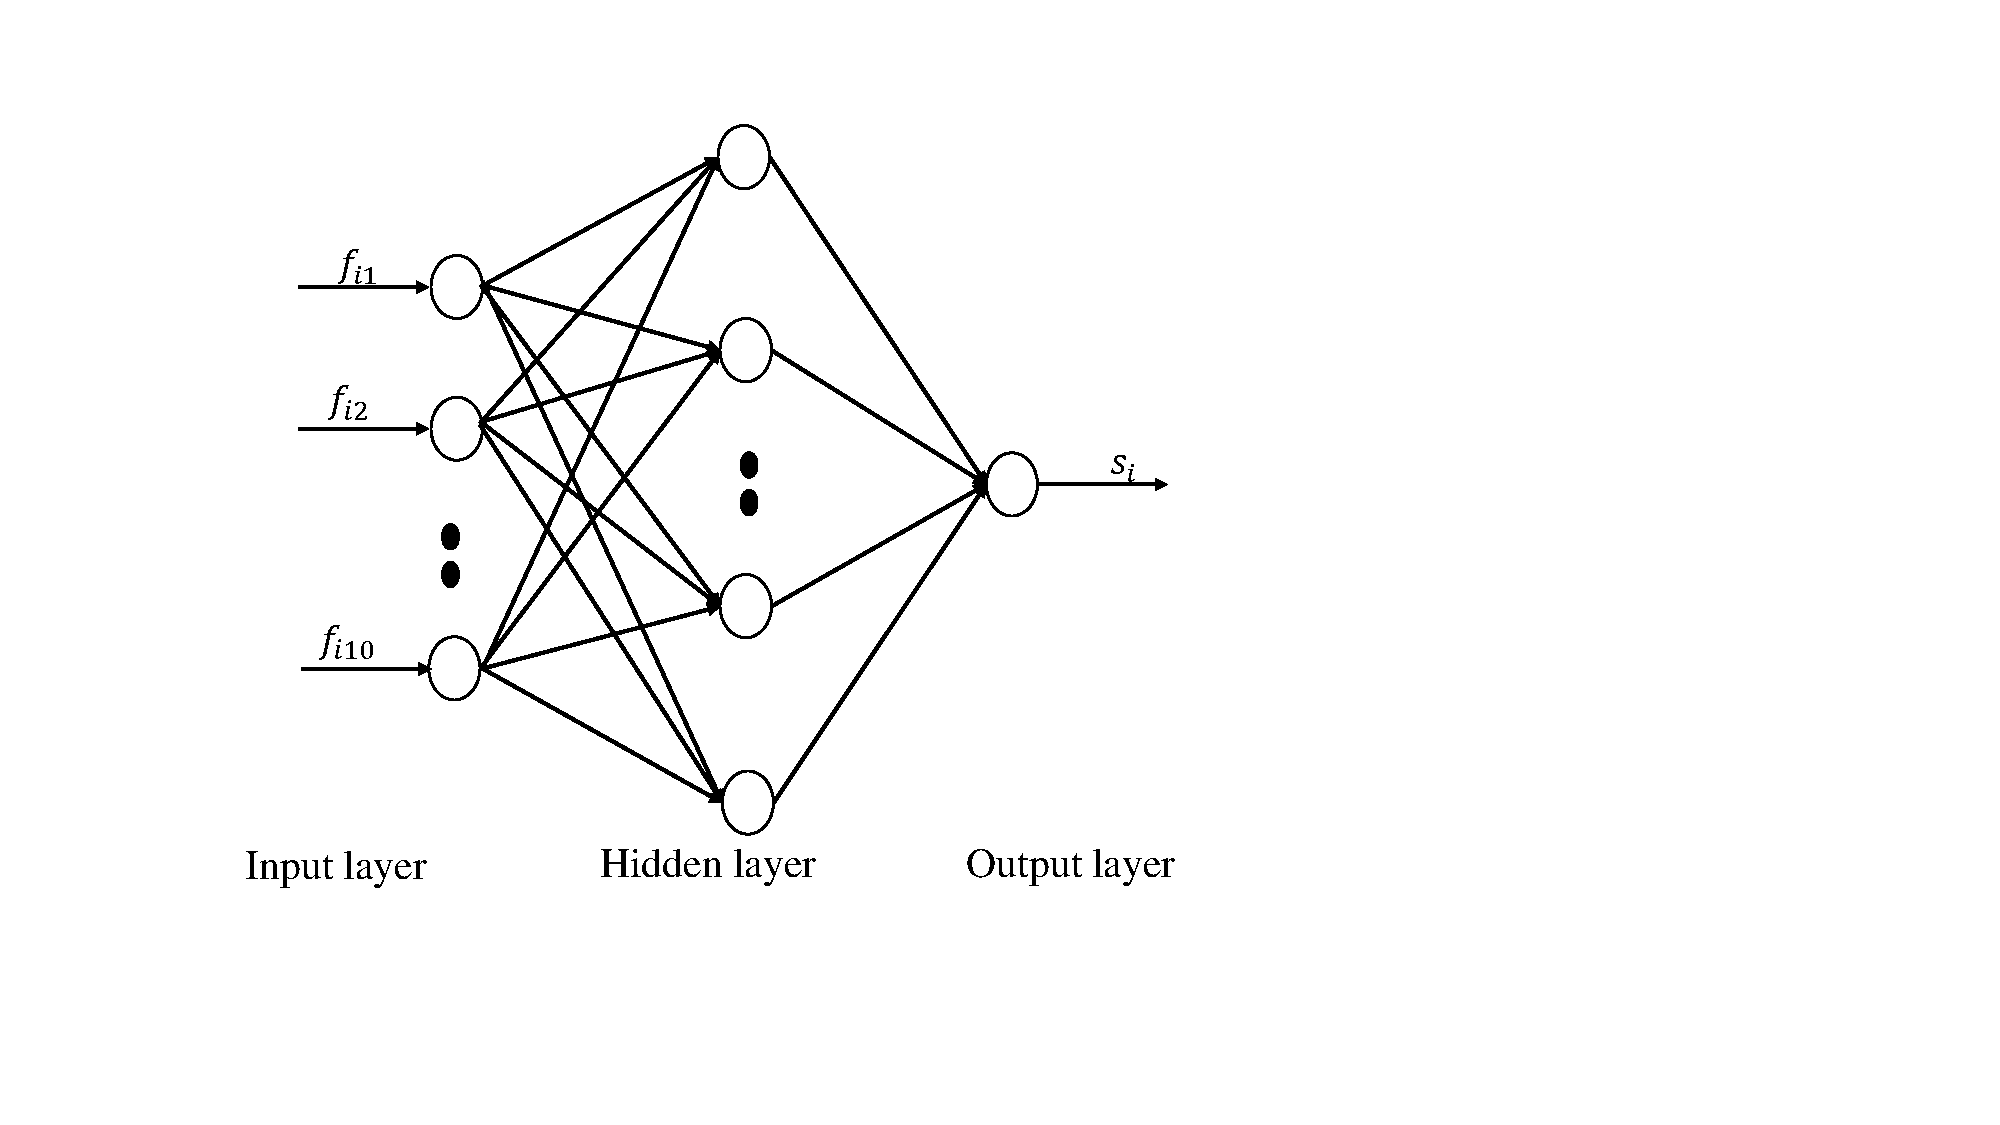
\includegraphics[width=0.6\linewidth]{bp}
		\caption{The Description of Multi-Feature Neural Ranking Model}
		\label{bp}
	\end{figure}
	
	We design a three layers neural network, as Fig.~\ref{bp}, this model is a gradient descent method designed to minimize the total error of predicted score and human rated score.
	The input layer is all features of each question. The middle layer is a hidden layer with $K$ nodes, and the last layer is the predicted score. $f_{ij}$ is $j$th feature of $i$th question. Furthermore, the multi-feature neural model is viewed as statistical model of the under form:
	\begin{equation}
		s_i = \beta_0+\sum_{j=1}^{K}\beta_j\Psi(w_jf_i)
	\end{equation}
	Where $i=1,2,...,M$, $M $ is the total number of training questions, $f$ is the set of features, $ \beta_j $ is the weight between layers, $s$ is the predicted score, $ \Psi$ is a non-linear squashing function like the rectified linear unit function:
	\begin{equation}
		\Psi(z)= \frac{1}{1+exp(-z)}
	\end{equation}
	And we use the mean square error $ e $ as loss function, that is:
	\begin{equation}
		e = \frac{1}{2M}\sum_{i=1}^{M}(t_i-p_i)^2
	\end{equation}
	
	Where $ t_i $ is the $i$-th actual score by human rated. We use a gradient descent method to reduce $ e $. When $ e < \varepsilon$, the neural network will be constructed, which can be used to compute the score of each question. Besides, by descending these scores attached to questions, we can obtain the top questions which are more acceptable by users.

		
	
	
	
	
	\section{Experiments}
	We conduct extensive experiments to evaluate the feasibility and effectiveness of our framework, and compare it with the state-of-the-art question generation systems.
	\subsection{Experimental Setup}
	We crawl ten topics of news data from Netease\footnote{http://news.163.com/} and Toutiao \footnote{https://www.toutiao.com/}, which are the popular Chinese media and website. The news contains ten topics, such as Economic (Ec), House, National, Military, Woman, Cars, Sports, Web, Entertainment (En), and Others. \revised{There are two hundred media news totally in the dataset \footnote{https://github.com/hanjx16/question-data.git}.} For each news topic, 80\% news are selected randomly as the training set, the rest news is used as the testing set.
	
	There are some parameters to setup before generating. In the adopted TextRank, the parameter $ d $ is usually set to 0.85 \cite{textrank}, and this is the value we are also using in our implementation; the threshold $ \theta $ is 1.2, which is a little greater than the independent sentence score. 
	In neural ranking model, the parameter $ K,\varepsilon$ are set to 5, 0.01 \cite{neural} respectively. These values can ensure the model is robust.
	For sentences analysis, we apply the Stanford CoreNLP \cite{stanford} to handle sentences including named entity recognizer and parser tree building. 
	
	\revised{
	We introduce three recent methods including H\&S, HSKS and HSMF for comparison to evaluate the performance of each framework. The compared methods are listed as follows:
	\begin{itemize}
		\item[$\bullet$]{H\&S: H\&S transforms the input sentence into a simpler sentence and the simpler sentence is transformed into sets of questions by a sequence of well-defined syntactic and lexical transformations.\cite{heilman2010good}} 
		\item[$\bullet$]{HSKS: HSKS extracts  the key sentences from texts and then constructs questions from the key sentences using templates.}
		\item[$\bullet$]{HSMF: HSMF applies a multi-feature model to rank all generated questions to make the top questions more useful.}
	\end{itemize}
}
	
	We calculate the perplexity \cite{Popel} score of generated questions, which is used to compare probability for nature language processing. Note that the lower perplexity indicates the generated questions are more likely to human writing.
	Besides, we also use human evaluation that is frequently adopted in recent works about question generation \cite{DBLP:journals/corr/DuSC17,Susanti2017,lindberg2013generating}. In human evaluation, all generated questions mixed together are evaluated by human, and each question is rated by two people. In detail, we define an evaluation criterion of question with different score values.
	\begin{itemize}
		\item[$\bullet$]{\emph{Good} represents the question is related to the text well without grammatical error and its score is 3.}
		\item[$\bullet$]{\emph{Borderline} represents the question has no problem from the view of the question but the answer does not make much sense (e.g., feature, today) and its score is 2.}
		\item[$\bullet$]{\emph{Bad} represents the question is redundant or the answer is a part of other question and its score is 1.}
	\end{itemize}
	
	
	
	\subsection{Experimental Results}
	
	
	Table.~\ref{perplexity} shows the perplexity score of $ n $-gram in each framework. Unigram is $n=1$, Bigram is $ n=2$ and Trigram is $n=3$. ACQG outperforms other frameworks, whose perplexity scores are 654.28 (Unigram), 418.46 (Bigram) and 166.53 (Trigram). H\&S uses the over-generated questions and ranks them to get the output questions. The full text is used to generate questions, thereby the outputs are redundant and the scores are 841.39 (Unigram), 608.21 (Bigram) and 213.34 (Trigram). HSKS filters unmeaning sentences in texts, which is able to generate more targeted questions. Thus the scores decrease dramatically. Referring to HSMF system, HSMF is superior to H\&S slightly. However the score of unigram is greater than H\&S. The reason is that they both construct more absurd questions and the ranking method cannot improve this issue effectively. When we improve both key sentence extracting and question ranking, the performance of ACQG achieves best.
	\begin{table}[!ht]
		\centering
		\caption{The Perplexity Score of $n$-gram in Different Frameworks}
		\label{perplexity}
		\setlength\tabcolsep{0.5em}
		\begin{tabular}{|p{50pt}|p{50pt}p{50pt}p{50pt}|}
			\hline
			Frameworks& Unigram & Bigram & Trigram \\
			\hline
			H\&S & 841.39 & 608.21 & 213.34\\
			HSKS & 735.42 & 464.62 & 187.25 \\
			HSMF& 821.8 & 584.42 & 205.72 \\
			ACQG & \textbf{654.28} & \textbf{418.46} & \textbf{166.53} \\
			\hline
		\end{tabular}
	\end{table}
	
	
	Furthermore, we introduce human evaluation into this work. The average marking scores are shown in Table.~\ref{averagescre} , the detailed score distribution in each topic is shown in Fig.~\ref{classcore}. 
	
	
	\begin{table}[!ht]
		\centering
		\caption{The Average Score of Human Evaluation in Different Frameworks}
		\label{averagescre}
		\setlength\tabcolsep{0.5em}
		\begin{tabular}{|p{80pt}|p{40pt}p{40pt}p{40pt}p{40pt}|}
			\hline
			Frameworks  & H\&S & HSKS & HSMF & ACGQ \\
			\hline
			Average Score & 1.79 & 2.12 & 1.95 &\textbf{2.37}\\
			\hline
		\end{tabular}
	\end{table}
	%1.79 2.06 1.91 2.32
	
	\revised{From Table.~\ref{averagescre}, we can see ACGQ has the highest score 2.37, which indicates that the generated questions are around \emph{Good} and \emph{Borderline}. The questions are more likely to be acceptable. Because of the bad input and fragile ranking method, H\&S has a poor performance, whose human evaluation score is only 1.79. 
	For HSKS and HSMF, whose human evaluation score are 2.12 and 1.95 respectively. They both show better performance than H\&S, but perform worse than ACGQ. Thus, the results of human evaluation are consistent with the above automatic evaluation.}
	%For only changing the input as HSKS, the questions improve a lot. Although the perplexity of unigram score is greater than H\&S, the human elevation result shows its function. The HSMF and H\&S results are both around \emph{Bad} and \emph{Borderline}, the only ranking method could only improve a little.  
	
	\begin{figure}[!ht]
		\centering
		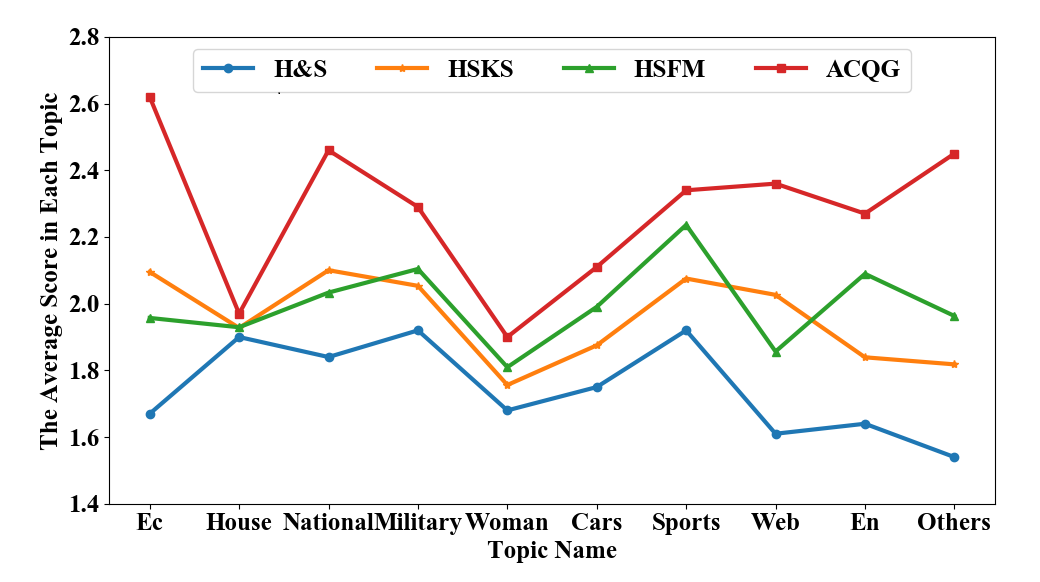
\includegraphics[width=0.7\linewidth]{score}
		\caption{The Human Evaluation in Each Topic}
		\label{classcore}
	\end{figure}
	
	
	%	\begin{figure}[!ht]
	%		\centering
	%		\includegraphics[width=0.6\linewidth]{sa.pdf}
	%		\caption{The Cumulative Distribution of Score }
	%		\label{sa}
	%	\end{figure}
	
	Fig.~\ref{classcore} shows the detailed human evaluation score distribution in each topic. We can observe that all frameworks have a low satisfaction score in the topic of House. The reason is that the collected news is almost advertisements in House, which cannot generate meaningful questions. For other topics, H\&S always shows a lower score in each topic, while ACQG always shows a higher score in each topic. For other frameworks, the results fluctuate within H\&S and ACQG. In detail, the upper scores are 2.62 (Ec), 1.97(House), 2.46 (National), 2.29 (Military), 1.90 (Woman), 2.11 (Cars), 2.34 (Sports), 2.36 (Web), 2.27 (En), 2.45 (Others) respectively. HSKS pays attention to the main points of text, which filters some noisy sentences from verbose text, so the generated questions almost match texts well. HSMF takes enough features into account, which makes the ranking model effective, thus the top questions are more likely acceptable. ACGQ includes both improved components, so we can see the average score of ACQG by human evaluation is the highest. Therefore, ACQG works effectively by extracting key sentences instead of full text and improving ranking method.
	
	
	%	Figure \ref{sa} shows the results of the human evaluation score distribution. The cumulative distribution of score in ACGQ are: 14.76\% (score $>=$ 3),28\% (score $>=$ 2.6), 58.76\% (score $>=$ 2.2), 84.87\% (score $>=$ 1.8), 93.8\% (score $>=$ 1.4) and 100\% (score $>=$ 1).
	
	%and the percentage of questions generated outperforms in each score stage by ACQG.
	
	
	
	
	%	\subsection{Error Analysis}
	%Analysis of unacceptable questions reveals both sources of errors and areas for future work. 
	%	Analysis of unacceptable questions reveals sources of errors and promotes the future work. Some errors are caused by inexact name entities. As person is regarded as a general entity by mistake. For the sentence \emph{``校长参加了这次开学典礼。(The headmaster attended the opening ceremony.)"}, the acceptable question is \emph{``谁参加了开幕式?(Who attended the opening ceremony?)"}, but if the headmaster is regarded as a general noun mistakenly in Chinese, the generated question will become \emph{``什么参加了开幕式?(what attended the open ceremony?)"}. One way to avoid generating this kind of questions would be to build a large named entity in Chinese and ensure we can find each name accurately.
	
	%	Another issue is that a template do not always work well in all topics. For example, a sentence \emph{``我们班里有50个学生。(There are 50 students in our class.)"},  The question matches the number template could be generated as \emph{``我们班有多少学生?(How many students in your class?)"}. However it will perform badly in other topics, a sentence  \emph{``1949年10月1日新中国成立了。(The People's Republic of China was founded in October 1, 1949)"}. The unacceptable question matches the number template is generated \emph{``多少年10月1日新中国成立了。(How many year the People's Republic of China was founded in October 1?)"}. However, an acceptable question is \emph{``什么时候新中国成立?(When was the People's Republic of China found?)"}.As the number of student in the first example is only one number, while the numbers in the second example should belongs to $When$ type of question, thus, it is necessary to select different templates for different topics of text or paragraph.
	
	\section{Conclusion and Future Work}
	%\section{Conclusion}
	We have proposed an automatic Chinese question generation framework (ACQG), a novel framework that generates more meaningful questions automatically to help readers obtain the main content of Chinese text. We use key sentences rather than the full content to generate questions, and then a template-based method is built to construct more variant questions. Finally, these questions are ranking by an efficient ranking method that leverages a multi-feature neural model to solve the multiple features problem. Extensive experiments are conducted on a Chinese dataset from the popular Chinese website and media, and the results show a significant improvement in terms of perplexity and human evaluation comparing with the baseline methods. We believe the proposed method will play an important role in question generation. 
	
	\revised{
		There  still exist limitations in ACGQ. For example,the types of generated questions are limited,which is caused by the limited templates.
		In the future work, we will design more useful templates from texts to generate more meaningful questions. In addition, we will construct enough pairs of text and questions to train an end-to-end neural model to generate high-quality Chinese questions directly.}
	
	
	\section{Acknowledgments}
	
	
	This research is supported by National Natural Science Foundation of China (Grant No. 61773229), Natural Science Foundation of Guangdong Province (Grant No. 2014A030313745), Basic Scientific Research Program of Shenzhen City (Grant No. JCYJ20160331184440545), and Cross fund of Graduate School at Shenzhen, Tsinghua University (Grant No. JC20140001).
	
	
	\bibliographystyle{splncs03}
	\bibliography{demo}
	


	
	
\end{document}
	